\section{Problem Statement and Method Summary}
The problem is the real-time implementation of spectral clustering algorithm of high dimensional embedding features which achieves top performance for the task of speaker diarisation but is hard to implement in a streaming mode as requiring full matrix operations on Laplacian kernel matrix. This TD proposes a novel iterative way to conduct that operations by applying a trick in cosine similarity kernel decomposition, making it to a tractable form expression to the mathematical problem, to enable the implementation in an iterative streaming fashion and also possible to further adoptions of Krylov low-rank approximation making it even faster and more accurate.

\section{Spectral Clustering}
Let $X \in \R^{n \times m}$ be the data matrix and a similarity function $k: \R^m \times \R^m \to [0, \infty)$. \textit{Spectral Clustering} constructs the similarity matrix $W \in \R^{n \times n}$ where each entry $W_{i j} = k(x_i, x_j)$. The Laplacian matrix is then calculated as $\mathcal{L} = I - D^{-1/2} W D^{-1/2}$. Based on \textit{Spectral Graph Theory}, the first $K$ eigenvectors of $\mathcal{L}$ well represents data under the similarity function $k$. \textit{K-means} is then used to form clusters from eigenvectors of $\mathcal{L}$.

\section{Streaming Spectral Clustering with Block Krylov Iteration}

Figure \ref{fig:spectral} shows the difference between \textit{Streaming Spectral Clustering} and \textit{Offline Spectral Clustering}.

\begin{figure}[htb]
    \begin{minipage}[b]{1.0\linewidth}
    \centering
    \centerline{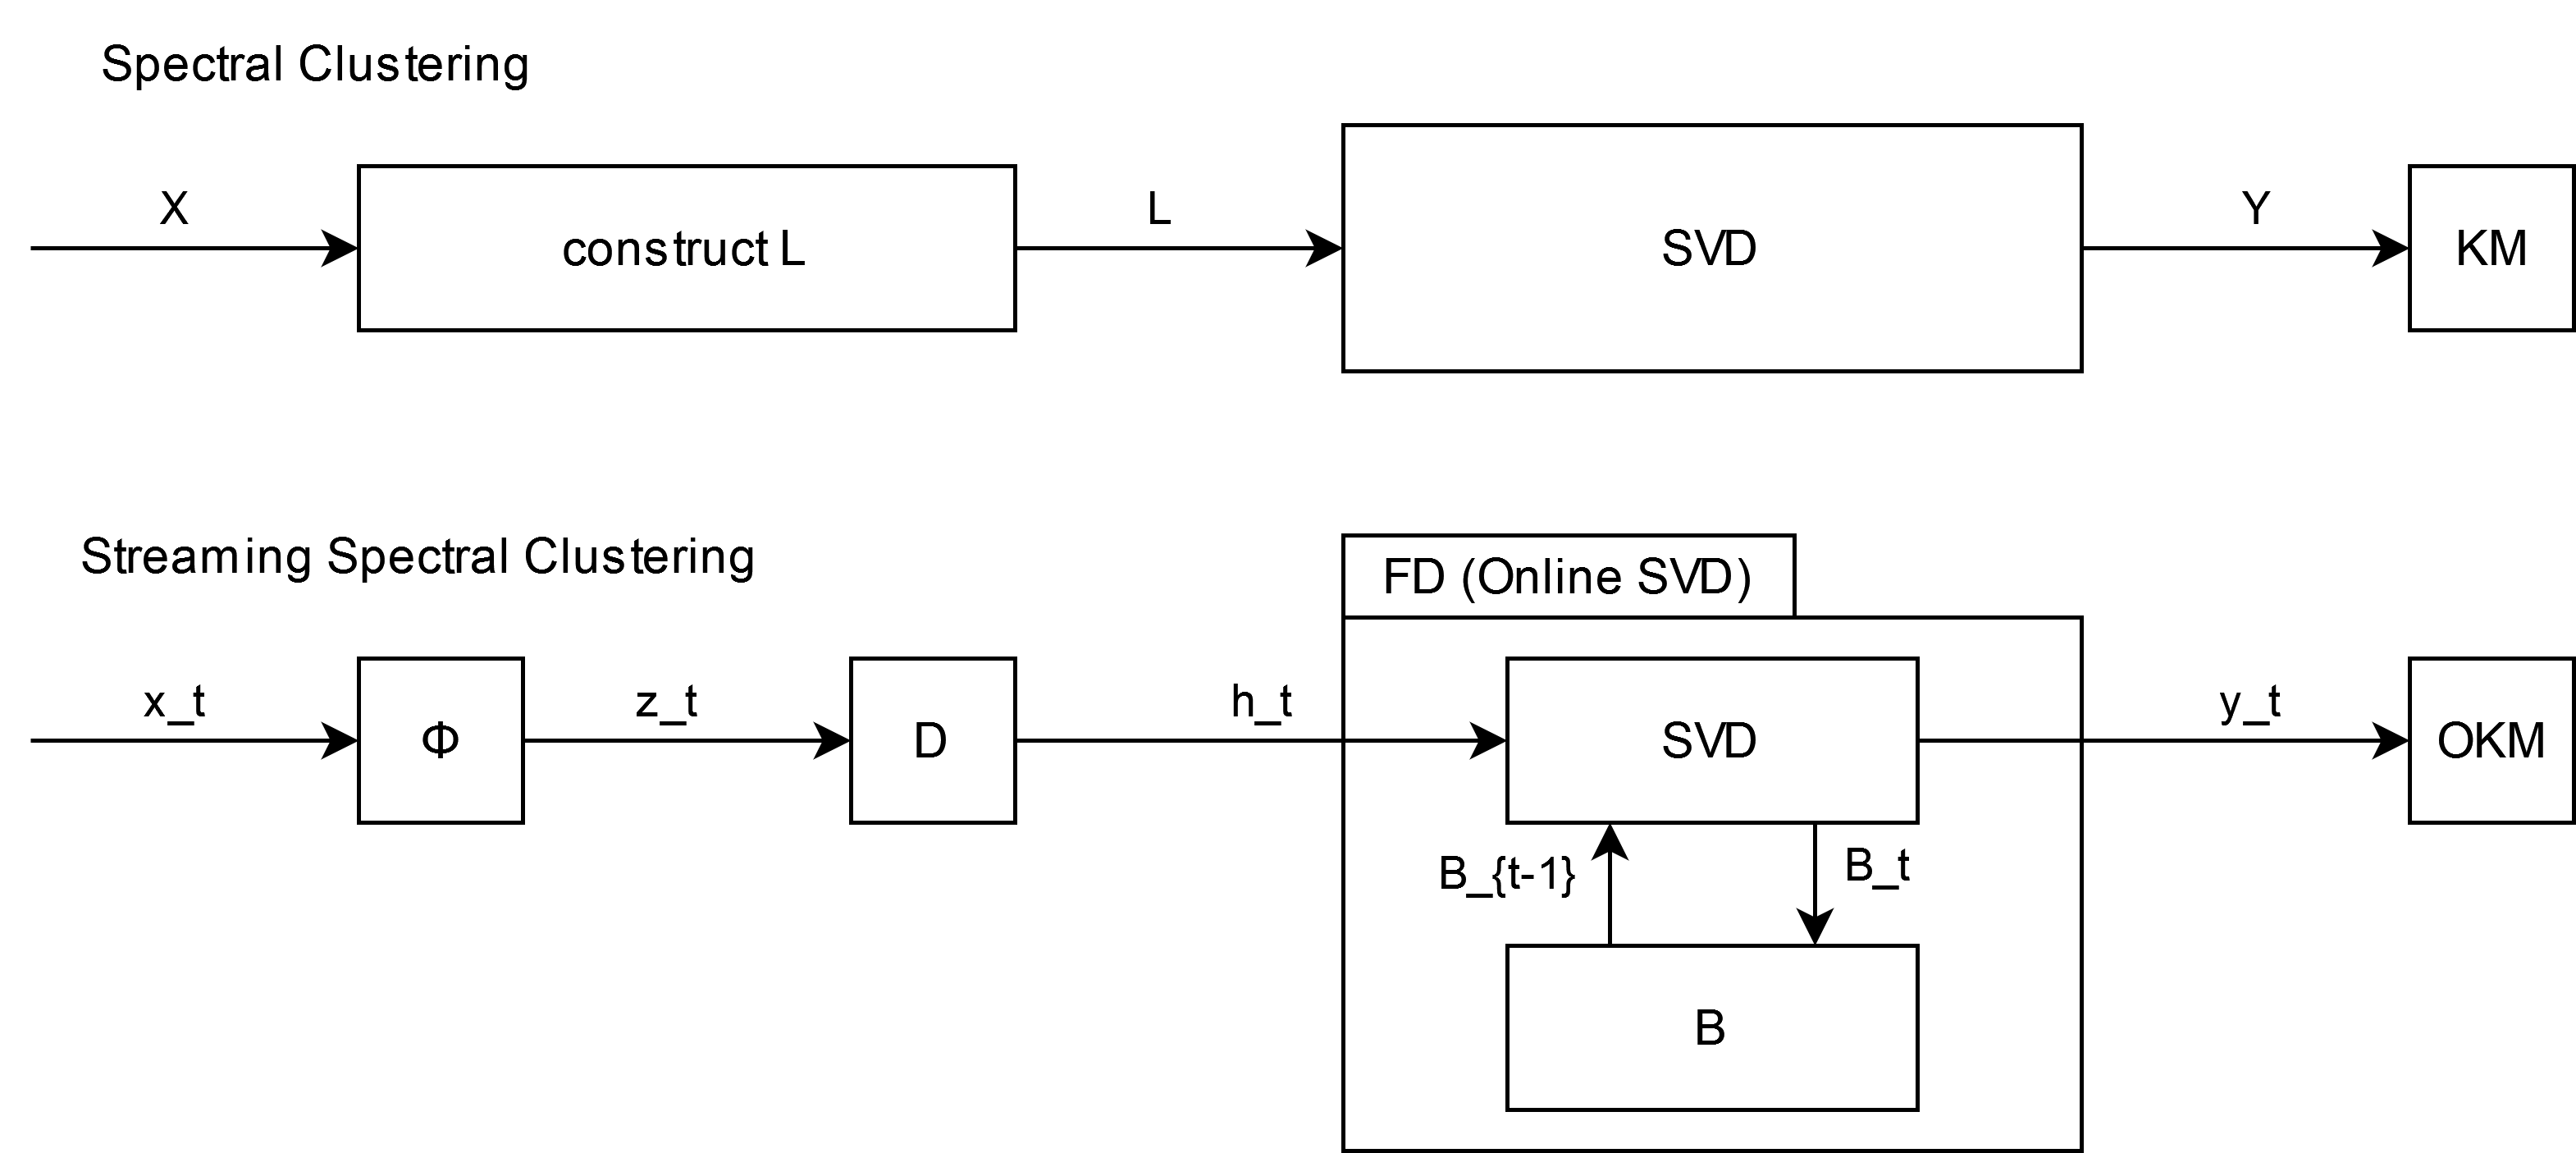
\includegraphics[width=8.5cm]{assets/ssc_diagram.png}}
    %\vspace{2.0cm}
    \end{minipage}
\caption{Speaker Diarization Pipeline}
\label{fig:spectral}
\end{figure}

In the online setup, let $X \in \R^{n \times m}$ be the data matrix where each row $x_t \in \R^{m}, t=1, 2, ..., n$ is recorded sequentially and a similarity function $k: \R^m \times \R^m \to [0, \infty)$ that is also a kernel. A neat update of the Cholesky decomposition of the Laplacian matrix is presented below.

\subsection{Kernel mapping function ($\phi$)}

Let the similarity function be the cosine function. 
$$
    k(x, y) = \frac{\langle x, y\rangle}{||x||.||y||}
$$
The kernel mapping function $\phi$ transforms each data point $x_t \in \R^m$ into $z_t \in \R^d$ such that $\langle z_i, z_j \rangle = k(x_i, x_j)$. For cosine, the kernel mapping function is
$$
    z_t = \phi(x_t) = \left(1, \frac{x_t^{(1)}}{||x_t||}, \frac{x_t^{(2)}}{||x_t||}, ..., \frac{x_t^{(m)}}{||x_t||}\right) \in \R^{m+1}
$$

\subsection{Degree Matrix Approximation (D)}

After that, normalizing $z_t$ according to the approximated degree matrix as 
$$
    h_t = D(z_t) \approx \frac{z_t}{\sqrt{\langle z_t, c_t \rangle}}
$$
where $c_t = (\sum_{j=1}^t z_j) / ||\sum_{j=1}^t z_j||$. That yields  rows of a matrix $H = (h_1, h_2, ..., h_n)$. The left singular vectors of $H$ coincide with the eigen vectors of the normalized Laplacian $\mathcal{L}$, which enables us to calculate eigenvectors of $\mathcal{L}$ in an online manner by calculating singular vectors of $H$ sequentially.

\subsection{Frequent Direction with Block Krylov Iteration (FD\_BKI)}

FD\_BKI (Algorithm \ref{alg:fd_bki}) is an extension of FD that is used to extract left singular vectors of $H$ sequentially. FD maintains a compression of the stream of data at time $t-1$ by a sketch matrix $B_{t-1} \in \R^{l \times d}$. When a new data point $h_t$ arrives, SVD algorithm is then used to extract the embedding of the $h_t$ sequentially. FD\_BKI adds an additional step (4-6) that both denoises and compresses the input $h_t$ based on the theory of Krylov subspace and Chebyshev polynomials.

\subsection{Online K-means (OKM)}

Similar to \textit{Offline Spectral Clustering}, \textit{Online K-means} is used to form clusters from singular vectors of $H$ in an online manner.


\begin{algorithm}
\caption{BKI \cite{musco2015randomized}}\label{alg:bki}
\begin{algorithmic}[1]
\Require $A \in \R^{n \times d}$, error $\epsilon > 0$, sketch size $l \leq n, d$
\Ensure $Z \in \R^{n \times l}$, $P \in \R^{l \times d}$
\State $q \gets \Theta(\frac{\log d}{\sqrt{\epsilon}})$, $\Pi \sim \mathcal{N}(0, 1)^{d \times l}$
\State $K \gets [A\Pi, (AA^T) A\Pi, ..., (AA^T)^{q-1} A\Pi] \in \R^{n \times lq}$
\State Orthonormalize columns of $K$ to obtain $Q \in \R^{n \times lq}$
\State Set $U_l \in \R^{lq \times l}$ to be the top-$l$ left singular vectors of $Q^T A$
\State $Z \gets Q U_l$, $P \gets Z^T A$
\end{algorithmic}
\end{algorithm}

\begin{algorithm}
\caption{FD \cite{yoo2016streaming} and FD\_BKI}\label{alg:fd_bki}
\begin{algorithmic}[1]
\Require $H = \{P_t \in \R^{b \times d} \}$, error $\epsilon > 0$, sketch size $l \ll d$, batch size $b$, output dimension $k \leq l$
\Ensure $Y = \{U_t \in \R^{b \times k} \}$, $V_t$

\State $B \gets \text{empty matrix} \in \R^{0 \times d}$

\While{stream $H$ is not empty}
    \State Read $b$ rows from $H$ to obtain $P_t \in \R^{b \times d}$
    \If{BKI is specified to use and $b > l$}
        \State $P_t \gets \text{BKI}(P_t, \epsilon, l)$ 
    \EndIf
    \State Append $P_t$ into $B$
    % \State  $U_t, V_t \gets \text{FD\_EXTRACT}(B, P_t)$
    \State $U, \Sigma, V \gets \text{SVD}(B)$
    \State $V_t \gets V_{[k]}, U_t \gets P_t V_{[k]} \Sigma_{[k]}^{-1}$
    \If{number of rows of $B \geq 2l$}
        % \State $B \gets \text{FD\_PRUNE}(B)$
        \State $\Bar{\Sigma} \gets \diag \left( \sqrt{\max \{0, \sigma^2 - \sigma_l^2\}}\right)$
        \State $B \gets \Bar{\Sigma}_{[l]} V_{[l]}^T$
    \EndIf
\EndWhile

\end{algorithmic}
\end{algorithm}